\documentclass[twoside]{book}

% Packages required by doxygen
\usepackage{fixltx2e}
\usepackage{calc}
\usepackage{doxygen}
\usepackage[export]{adjustbox} % also loads graphicx
\usepackage{graphicx}
\usepackage[utf8]{inputenc}
\usepackage{makeidx}
\usepackage{multicol}
\usepackage{multirow}
\PassOptionsToPackage{warn}{textcomp}
\usepackage{textcomp}
\usepackage[nointegrals]{wasysym}
\usepackage[table]{xcolor}

% Font selection
\usepackage[T1]{fontenc}
\usepackage[scaled=.90]{helvet}
\usepackage{courier}
\usepackage{amssymb}
\usepackage{sectsty}
\renewcommand{\familydefault}{\sfdefault}
\allsectionsfont{%
  \fontseries{bc}\selectfont%
  \color{darkgray}%
}
\renewcommand{\DoxyLabelFont}{%
  \fontseries{bc}\selectfont%
  \color{darkgray}%
}
\newcommand{\+}{\discretionary{\mbox{\scriptsize$\hookleftarrow$}}{}{}}

% Page & text layout
\usepackage{geometry}
\geometry{%
  a4paper,%
  top=2.5cm,%
  bottom=2.5cm,%
  left=2.5cm,%
  right=2.5cm%
}
\tolerance=750
\hfuzz=15pt
\hbadness=750
\setlength{\emergencystretch}{15pt}
\setlength{\parindent}{0cm}
\setlength{\parskip}{3ex plus 2ex minus 2ex}
\makeatletter
\renewcommand{\paragraph}{%
  \@startsection{paragraph}{4}{0ex}{-1.0ex}{1.0ex}{%
    \normalfont\normalsize\bfseries\SS@parafont%
  }%
}
\renewcommand{\subparagraph}{%
  \@startsection{subparagraph}{5}{0ex}{-1.0ex}{1.0ex}{%
    \normalfont\normalsize\bfseries\SS@subparafont%
  }%
}
\makeatother

% Headers & footers
\usepackage{fancyhdr}
\pagestyle{fancyplain}
\fancyhead[LE]{\fancyplain{}{\bfseries\thepage}}
\fancyhead[CE]{\fancyplain{}{}}
\fancyhead[RE]{\fancyplain{}{\bfseries\leftmark}}
\fancyhead[LO]{\fancyplain{}{\bfseries\rightmark}}
\fancyhead[CO]{\fancyplain{}{}}
\fancyhead[RO]{\fancyplain{}{\bfseries\thepage}}
\fancyfoot[LE]{\fancyplain{}{}}
\fancyfoot[CE]{\fancyplain{}{}}
\fancyfoot[RE]{\fancyplain{}{\bfseries\scriptsize Generated by Doxygen }}
\fancyfoot[LO]{\fancyplain{}{\bfseries\scriptsize Generated by Doxygen }}
\fancyfoot[CO]{\fancyplain{}{}}
\fancyfoot[RO]{\fancyplain{}{}}
\renewcommand{\footrulewidth}{0.4pt}
\renewcommand{\chaptermark}[1]{%
  \markboth{#1}{}%
}
\renewcommand{\sectionmark}[1]{%
  \markright{\thesection\ #1}%
}

% Indices & bibliography
\usepackage{natbib}
\usepackage[titles]{tocloft}
\setcounter{tocdepth}{3}
\setcounter{secnumdepth}{5}
\makeindex

% Hyperlinks (required, but should be loaded last)
\usepackage{ifpdf}
\ifpdf
  \usepackage[pdftex,pagebackref=true]{hyperref}
\else
  \usepackage[ps2pdf,pagebackref=true]{hyperref}
\fi
\hypersetup{%
  colorlinks=true,%
  linkcolor=blue,%
  citecolor=blue,%
  unicode%
}

% Custom commands
\newcommand{\clearemptydoublepage}{%
  \newpage{\pagestyle{empty}\cleardoublepage}%
}

\usepackage{caption}
\captionsetup{labelsep=space,justification=centering,font={bf},singlelinecheck=off,skip=4pt,position=top}

%===== C O N T E N T S =====

\begin{document}

% Titlepage & ToC
\hypersetup{pageanchor=false,
             bookmarksnumbered=true,
             pdfencoding=unicode
            }
\pagenumbering{roman}
\begin{titlepage}
\vspace*{7cm}
\begin{center}%
{\Large kinect\+Expirement }\\
\vspace*{1cm}
{\large Generated by Doxygen 1.8.11}\\
\end{center}
\end{titlepage}
\clearemptydoublepage
\tableofcontents
\clearemptydoublepage
\pagenumbering{arabic}
\hypersetup{pageanchor=true}

%--- Begin generated contents ---
\chapter{Namespace Index}
\section{Packages}
Here are the packages with brief descriptions (if available)\+:\begin{DoxyCompactList}
\item\contentsline{section}{\hyperlink{namespacekinect_expirement}{kinect\+Expirement} }{\pageref{namespacekinect_expirement}}{}
\end{DoxyCompactList}

\chapter{Hierarchical Index}
\section{Class Hierarchy}
This inheritance list is sorted roughly, but not completely, alphabetically\+:\begin{DoxyCompactList}
\item \contentsline{section}{kinect\+Expirement.\+Arduino\+Control}{\pageref{classkinect_expirement_1_1_arduino_control}}{}
\item \contentsline{section}{kinect\+Expirement.\+Butterworth}{\pageref{classkinect_expirement_1_1_butterworth}}{}
\item \contentsline{section}{kinect\+Expirement.\+Calculate}{\pageref{classkinect_expirement_1_1_calculate}}{}
\item \contentsline{section}{kinect\+Expirement.\+Encoder\+Sensor\+Class}{\pageref{classkinect_expirement_1_1_encoder_sensor_class}}{}
\item \contentsline{section}{kinect\+Expirement.\+File\+Processing}{\pageref{classkinect_expirement_1_1_file_processing}}{}
\item Form\begin{DoxyCompactList}
\item \contentsline{section}{kinect\+Expirement.\+Kinect\+Form}{\pageref{classkinect_expirement_1_1_kinect_form}}{}
\end{DoxyCompactList}
\item \contentsline{section}{kinect\+Expirement.\+Kinect\+Sensor\+Class}{\pageref{classkinect_expirement_1_1_kinect_sensor_class}}{}
\item \contentsline{section}{kinect\+Expirement.\+Point\+Holder}{\pageref{classkinect_expirement_1_1_point_holder}}{}
\end{DoxyCompactList}

\chapter{Class Index}
\section{Class List}
Here are the classes, structs, unions and interfaces with brief descriptions\+:\begin{DoxyCompactList}
\item\contentsline{section}{\hyperlink{classkinect_expirement_1_1_arduino_control}{kinect\+Expirement.\+Arduino\+Control} \\*Contains functions for reading in values from the Arduino. }{\pageref{classkinect_expirement_1_1_arduino_control}}{}
\item\contentsline{section}{\hyperlink{classkinect_expirement_1_1_butterworth}{kinect\+Expirement.\+Butterworth} \\*A butterworth filter for the values taken from the Kinect and encoder.}{\pageref{classkinect_expirement_1_1_butterworth}}{}
\item\contentsline{section}{\hyperlink{classkinect_expirement_1_1_calculate}{kinect\+Expirement.\+Calculate} \\*Holds all the calculation functions.}{\pageref{classkinect_expirement_1_1_calculate}}{}
\item\contentsline{section}{\hyperlink{classkinect_expirement_1_1_encoder_sensor_class}{kinect\+Expirement.\+Encoder\+Sensor\+Class} \\*Handles all of the functions for dealing with values from the encoder. }{\pageref{classkinect_expirement_1_1_encoder_sensor_class}}{}
\item\contentsline{section}{\hyperlink{classkinect_expirement_1_1_file_processing}{kinect\+Expirement.\+File\+Processing} \\*Controls all the file processing.}{\pageref{classkinect_expirement_1_1_file_processing}}{}
\item\contentsline{section}{\hyperlink{classkinect_expirement_1_1_kinect_form}{kinect\+Expirement.\+Kinect\+Form} \\*Inheriated from Form class, G\+UI for incoder and Kinect handling. }{\pageref{classkinect_expirement_1_1_kinect_form}}{}
\item\contentsline{section}{\hyperlink{classkinect_expirement_1_1_kinect_sensor_class}{kinect\+Expirement.\+Kinect\+Sensor\+Class} \\*Holds all the functions for reading in and storeing values from the Kinect, also constrols the state of the sensor. }{\pageref{classkinect_expirement_1_1_kinect_sensor_class}}{}
\item\contentsline{section}{\hyperlink{classkinect_expirement_1_1_point_holder}{kinect\+Expirement.\+Point\+Holder} \\*Holds the x,y and z positions of a point. }{\pageref{classkinect_expirement_1_1_point_holder}}{}
\end{DoxyCompactList}

\chapter{Namespace Documentation}
\hypertarget{namespacekinect_expirement}{}\section{kinect\+Expirement Namespace Reference}
\label{namespacekinect_expirement}\index{kinect\+Expirement@{kinect\+Expirement}}
\subsection*{Classes}
\begin{DoxyCompactItemize}
\item 
class \hyperlink{classkinect_expirement_1_1_arduino_control}{Arduino\+Control}
\begin{DoxyCompactList}\small\item\em Contains functions for reading in values from the Arduino. \end{DoxyCompactList}\item 
class \hyperlink{classkinect_expirement_1_1_butterworth}{Butterworth}
\begin{DoxyCompactList}\small\item\em A butterworth filter for the values taken from the Kinect and encoder.\end{DoxyCompactList}\item 
class \hyperlink{classkinect_expirement_1_1_calculate}{Calculate}
\begin{DoxyCompactList}\small\item\em Holds all the calculation functions.\end{DoxyCompactList}\item 
class \hyperlink{classkinect_expirement_1_1_encoder_sensor_class}{Encoder\+Sensor\+Class}
\begin{DoxyCompactList}\small\item\em Handles all of the functions for dealing with values from the encoder. \end{DoxyCompactList}\item 
class \hyperlink{classkinect_expirement_1_1_file_processing}{File\+Processing}
\begin{DoxyCompactList}\small\item\em Controls all the file processing.\end{DoxyCompactList}\item 
class \hyperlink{classkinect_expirement_1_1_kinect_form}{Kinect\+Form}
\begin{DoxyCompactList}\small\item\em Inheriated from Form class, G\+UI for incoder and Kinect handling. \end{DoxyCompactList}\item 
class \hyperlink{classkinect_expirement_1_1_kinect_sensor_class}{Kinect\+Sensor\+Class}
\begin{DoxyCompactList}\small\item\em Holds all the functions for reading in and storeing values from the Kinect, also constrols the state of the sensor. \end{DoxyCompactList}\item 
class \hyperlink{classkinect_expirement_1_1_point_holder}{Point\+Holder}
\begin{DoxyCompactList}\small\item\em Holds the x,y and z positions of a point. \end{DoxyCompactList}\end{DoxyCompactItemize}

\chapter{Class Documentation}
\hypertarget{classkinect_expirement_1_1_arduino_control}{}\section{kinect\+Expirement.\+Arduino\+Control Class Reference}
\label{classkinect_expirement_1_1_arduino_control}\index{kinect\+Expirement.\+Arduino\+Control@{kinect\+Expirement.\+Arduino\+Control}}


Contains functions for reading in values from the Arduino.  


\subsection*{Public Member Functions}
\begin{DoxyCompactItemize}
\item 
\hyperlink{classkinect_expirement_1_1_arduino_control_a958454e66f96b46352d143acc5890cfe}{Arduino\+Control} ()
\begin{DoxyCompactList}\small\item\em Opens the serial \end{DoxyCompactList}\item 
float \hyperlink{classkinect_expirement_1_1_arduino_control_a49f81b66981e080da2324c09671a0335}{read\+Serial} ()
\begin{DoxyCompactList}\small\item\em Reads in a float from the serial that was sent by the Arduino. \end{DoxyCompactList}\end{DoxyCompactItemize}


\subsection{Detailed Description}
Contains functions for reading in values from the Arduino. 



\subsection{Constructor \& Destructor Documentation}
\index{kinect\+Expirement\+::\+Arduino\+Control@{kinect\+Expirement\+::\+Arduino\+Control}!Arduino\+Control@{Arduino\+Control}}
\index{Arduino\+Control@{Arduino\+Control}!kinect\+Expirement\+::\+Arduino\+Control@{kinect\+Expirement\+::\+Arduino\+Control}}
\subsubsection[{\texorpdfstring{Arduino\+Control()}{ArduinoControl()}}]{\setlength{\rightskip}{0pt plus 5cm}kinect\+Expirement.\+Arduino\+Control.\+Arduino\+Control (
\begin{DoxyParamCaption}
{}
\end{DoxyParamCaption}
)}\hypertarget{classkinect_expirement_1_1_arduino_control_a958454e66f96b46352d143acc5890cfe}{}\label{classkinect_expirement_1_1_arduino_control_a958454e66f96b46352d143acc5890cfe}


Opens the serial 



\subsection{Member Function Documentation}
\index{kinect\+Expirement\+::\+Arduino\+Control@{kinect\+Expirement\+::\+Arduino\+Control}!read\+Serial@{read\+Serial}}
\index{read\+Serial@{read\+Serial}!kinect\+Expirement\+::\+Arduino\+Control@{kinect\+Expirement\+::\+Arduino\+Control}}
\subsubsection[{\texorpdfstring{read\+Serial()}{readSerial()}}]{\setlength{\rightskip}{0pt plus 5cm}float kinect\+Expirement.\+Arduino\+Control.\+read\+Serial (
\begin{DoxyParamCaption}
{}
\end{DoxyParamCaption}
)}\hypertarget{classkinect_expirement_1_1_arduino_control_a49f81b66981e080da2324c09671a0335}{}\label{classkinect_expirement_1_1_arduino_control_a49f81b66981e080da2324c09671a0335}


Reads in a float from the serial that was sent by the Arduino. 

\begin{DoxyReturn}{Returns}
A float value for the output of the Arduino. 
\end{DoxyReturn}


The documentation for this class was generated from the following file\+:\begin{DoxyCompactItemize}
\item 
Program.\+cs\end{DoxyCompactItemize}

\hypertarget{classkinect_expirement_1_1_butterworth}{}\section{kinect\+Expirement.\+Butterworth Class Reference}
\label{classkinect_expirement_1_1_butterworth}\index{kinect\+Expirement.\+Butterworth@{kinect\+Expirement.\+Butterworth}}


A butterworth filter for the values taken from the Kinect and encoder.  


\subsection*{Public Member Functions}
\begin{DoxyCompactItemize}
\item 
\hyperlink{classkinect_expirement_1_1_butterworth_a37322f18a1f8f59271df8aac36e79f26}{Butterworth} (bool input)
\begin{DoxyCompactList}\small\item\em Constructor for the butterworth class \end{DoxyCompactList}\item 
List$<$ double $>$ \hyperlink{classkinect_expirement_1_1_butterworth_a0e51ad9aa7218b63b901cfd4e71ea75b}{Filter} (List$<$ double $>$ x, List$<$ double $>$ prev)
\begin{DoxyCompactList}\small\item\em Filters the list of values. \end{DoxyCompactList}\end{DoxyCompactItemize}
\subsection*{Public Attributes}
\begin{DoxyCompactItemize}
\item 
const bool \hyperlink{classkinect_expirement_1_1_butterworth_afc717929ffc8d554b7e0263e2b06806a}{V\+E\+L\+O\+C\+I\+TY} = true
\begin{DoxyCompactList}\small\item\em Constant boolean for the constructor to set the list to values for filtering velcity. \end{DoxyCompactList}\item 
const bool \hyperlink{classkinect_expirement_1_1_butterworth_ac991123445c654cb0da7d7841e313b2c}{A\+N\+G\+LE} = false
\begin{DoxyCompactList}\small\item\em Constant boolean for the constructor to set the list to values for filtering velcity. \end{DoxyCompactList}\end{DoxyCompactItemize}


\subsection{Detailed Description}
A butterworth filter for the values taken from the Kinect and encoder. 



\subsection{Constructor \& Destructor Documentation}
\index{kinect\+Expirement\+::\+Butterworth@{kinect\+Expirement\+::\+Butterworth}!Butterworth@{Butterworth}}
\index{Butterworth@{Butterworth}!kinect\+Expirement\+::\+Butterworth@{kinect\+Expirement\+::\+Butterworth}}
\subsubsection[{\texorpdfstring{Butterworth(bool input)}{Butterworth(bool input)}}]{\setlength{\rightskip}{0pt plus 5cm}kinect\+Expirement.\+Butterworth.\+Butterworth (
\begin{DoxyParamCaption}
\item[{bool}]{input}
\end{DoxyParamCaption}
)}\hypertarget{classkinect_expirement_1_1_butterworth_a37322f18a1f8f59271df8aac36e79f26}{}\label{classkinect_expirement_1_1_butterworth_a37322f18a1f8f59271df8aac36e79f26}


Constructor for the butterworth class 



\subsection{Member Function Documentation}
\index{kinect\+Expirement\+::\+Butterworth@{kinect\+Expirement\+::\+Butterworth}!Filter@{Filter}}
\index{Filter@{Filter}!kinect\+Expirement\+::\+Butterworth@{kinect\+Expirement\+::\+Butterworth}}
\subsubsection[{\texorpdfstring{Filter(\+List$<$ double $>$ x, List$<$ double $>$ prev)}{Filter(List< double > x, List< double > prev)}}]{\setlength{\rightskip}{0pt plus 5cm}List$<$double$>$ kinect\+Expirement.\+Butterworth.\+Filter (
\begin{DoxyParamCaption}
\item[{List$<$ double $>$}]{x, }
\item[{List$<$ double $>$}]{prev}
\end{DoxyParamCaption}
)}\hypertarget{classkinect_expirement_1_1_butterworth_a0e51ad9aa7218b63b901cfd4e71ea75b}{}\label{classkinect_expirement_1_1_butterworth_a0e51ad9aa7218b63b901cfd4e71ea75b}


Filters the list of values. 


\begin{DoxyParams}{Parameters}
{\em x} & The list of values to be filtered. \\
\hline
{\em prev} & The list of previous values before {\ttfamily x} was being recorded. \\
\hline
\end{DoxyParams}
\begin{DoxyReturn}{Returns}
A list of filtered values. 
\end{DoxyReturn}


\subsection{Member Data Documentation}
\index{kinect\+Expirement\+::\+Butterworth@{kinect\+Expirement\+::\+Butterworth}!A\+N\+G\+LE@{A\+N\+G\+LE}}
\index{A\+N\+G\+LE@{A\+N\+G\+LE}!kinect\+Expirement\+::\+Butterworth@{kinect\+Expirement\+::\+Butterworth}}
\subsubsection[{\texorpdfstring{A\+N\+G\+LE}{ANGLE}}]{\setlength{\rightskip}{0pt plus 5cm}const bool kinect\+Expirement.\+Butterworth.\+A\+N\+G\+LE = false}\hypertarget{classkinect_expirement_1_1_butterworth_ac991123445c654cb0da7d7841e313b2c}{}\label{classkinect_expirement_1_1_butterworth_ac991123445c654cb0da7d7841e313b2c}


Constant boolean for the constructor to set the list to values for filtering velcity. 

\index{kinect\+Expirement\+::\+Butterworth@{kinect\+Expirement\+::\+Butterworth}!V\+E\+L\+O\+C\+I\+TY@{V\+E\+L\+O\+C\+I\+TY}}
\index{V\+E\+L\+O\+C\+I\+TY@{V\+E\+L\+O\+C\+I\+TY}!kinect\+Expirement\+::\+Butterworth@{kinect\+Expirement\+::\+Butterworth}}
\subsubsection[{\texorpdfstring{V\+E\+L\+O\+C\+I\+TY}{VELOCITY}}]{\setlength{\rightskip}{0pt plus 5cm}const bool kinect\+Expirement.\+Butterworth.\+V\+E\+L\+O\+C\+I\+TY = true}\hypertarget{classkinect_expirement_1_1_butterworth_afc717929ffc8d554b7e0263e2b06806a}{}\label{classkinect_expirement_1_1_butterworth_afc717929ffc8d554b7e0263e2b06806a}


Constant boolean for the constructor to set the list to values for filtering velcity. 



The documentation for this class was generated from the following file\+:\begin{DoxyCompactItemize}
\item 
C\+:/\+Users/\+Kyle/\+Documents/kinectc/kinect\+Expirement/Program.\+cs\end{DoxyCompactItemize}

\hypertarget{classkinect_expirement_1_1_calculate}{}\section{kinect\+Expirement.\+Calculate Class Reference}
\label{classkinect_expirement_1_1_calculate}\index{kinect\+Expirement.\+Calculate@{kinect\+Expirement.\+Calculate}}


Holds all the calculation functions. 


\subsection*{Static Public Member Functions}
\begin{DoxyCompactItemize}
\item 
static \hyperlink{classkinect_expirement_1_1_point_holder}{Point\+Holder} \hyperlink{classkinect_expirement_1_1_calculate_a8fdf801a3bdee7bd1a327cc42e86aed9}{Create\+Vector} (\hyperlink{classkinect_expirement_1_1_point_holder}{Point\+Holder} point1, \hyperlink{classkinect_expirement_1_1_point_holder}{Point\+Holder} point2)
\begin{DoxyCompactList}\small\item\em Takes two points and generate a vector between them in 3 dimensions. \end{DoxyCompactList}\item 
static double \hyperlink{classkinect_expirement_1_1_calculate_a9c9d55d2e89605013fd5280deb572468}{Vector\+Length} (\hyperlink{classkinect_expirement_1_1_point_holder}{Point\+Holder} vector)
\begin{DoxyCompactList}\small\item\em Calculates the length of the vector. \end{DoxyCompactList}\item 
static double \hyperlink{classkinect_expirement_1_1_calculate_a5e407f5e00cb311cea31f7172fa4a5d0}{Dot\+Product} (\hyperlink{classkinect_expirement_1_1_point_holder}{Point\+Holder} vector1, \hyperlink{classkinect_expirement_1_1_point_holder}{Point\+Holder} vector2)
\begin{DoxyCompactList}\small\item\em Calculates the dot product of two vectors. \end{DoxyCompactList}\item 
static double \hyperlink{classkinect_expirement_1_1_calculate_a02fbfb617abfb0e06c8e92cb25f9f9e8}{To\+Degree} (double value)
\begin{DoxyCompactList}\small\item\em Converts a value from radians to degrees. \end{DoxyCompactList}\item 
static double \hyperlink{classkinect_expirement_1_1_calculate_a91876175c733dc14e51ac1eb5c255142}{Find\+Velocity} (double inital\+\_\+angle, double final\+\_\+angle)
\begin{DoxyCompactList}\small\item\em Calculates the velocity of angle movement, assuming that the frequency is 30\+Hz. \end{DoxyCompactList}\end{DoxyCompactItemize}


\subsection{Detailed Description}
Holds all the calculation functions.



\subsection{Member Function Documentation}
\index{kinect\+Expirement\+::\+Calculate@{kinect\+Expirement\+::\+Calculate}!Create\+Vector@{Create\+Vector}}
\index{Create\+Vector@{Create\+Vector}!kinect\+Expirement\+::\+Calculate@{kinect\+Expirement\+::\+Calculate}}
\subsubsection[{\texorpdfstring{Create\+Vector(\+Point\+Holder point1, Point\+Holder point2)}{CreateVector(PointHolder point1, PointHolder point2)}}]{\setlength{\rightskip}{0pt plus 5cm}static {\bf Point\+Holder} kinect\+Expirement.\+Calculate.\+Create\+Vector (
\begin{DoxyParamCaption}
\item[{{\bf Point\+Holder}}]{point1, }
\item[{{\bf Point\+Holder}}]{point2}
\end{DoxyParamCaption}
)\hspace{0.3cm}{\ttfamily [static]}}\hypertarget{classkinect_expirement_1_1_calculate_a8fdf801a3bdee7bd1a327cc42e86aed9}{}\label{classkinect_expirement_1_1_calculate_a8fdf801a3bdee7bd1a327cc42e86aed9}


Takes two points and generate a vector between them in 3 dimensions. 


\begin{DoxyParams}{Parameters}
{\em point1} & The first point in three dimensional space. \\
\hline
{\em point2} & The second point in three dimensional space. \\
\hline
\end{DoxyParams}
\begin{DoxyReturn}{Returns}
The vector that was generated. 
\end{DoxyReturn}
\index{kinect\+Expirement\+::\+Calculate@{kinect\+Expirement\+::\+Calculate}!Dot\+Product@{Dot\+Product}}
\index{Dot\+Product@{Dot\+Product}!kinect\+Expirement\+::\+Calculate@{kinect\+Expirement\+::\+Calculate}}
\subsubsection[{\texorpdfstring{Dot\+Product(\+Point\+Holder vector1, Point\+Holder vector2)}{DotProduct(PointHolder vector1, PointHolder vector2)}}]{\setlength{\rightskip}{0pt plus 5cm}static double kinect\+Expirement.\+Calculate.\+Dot\+Product (
\begin{DoxyParamCaption}
\item[{{\bf Point\+Holder}}]{vector1, }
\item[{{\bf Point\+Holder}}]{vector2}
\end{DoxyParamCaption}
)\hspace{0.3cm}{\ttfamily [static]}}\hypertarget{classkinect_expirement_1_1_calculate_a5e407f5e00cb311cea31f7172fa4a5d0}{}\label{classkinect_expirement_1_1_calculate_a5e407f5e00cb311cea31f7172fa4a5d0}


Calculates the dot product of two vectors. 


\begin{DoxyParams}{Parameters}
{\em vector1} & The first three dimensional vector. \\
\hline
{\em vector2} & The second three dimensional vector \\
\hline
\end{DoxyParams}
\begin{DoxyReturn}{Returns}
The dot product of the two vectors. 
\end{DoxyReturn}
\index{kinect\+Expirement\+::\+Calculate@{kinect\+Expirement\+::\+Calculate}!Find\+Velocity@{Find\+Velocity}}
\index{Find\+Velocity@{Find\+Velocity}!kinect\+Expirement\+::\+Calculate@{kinect\+Expirement\+::\+Calculate}}
\subsubsection[{\texorpdfstring{Find\+Velocity(double inital\+\_\+angle, double final\+\_\+angle)}{FindVelocity(double inital_angle, double final_angle)}}]{\setlength{\rightskip}{0pt plus 5cm}static double kinect\+Expirement.\+Calculate.\+Find\+Velocity (
\begin{DoxyParamCaption}
\item[{double}]{inital\+\_\+angle, }
\item[{double}]{final\+\_\+angle}
\end{DoxyParamCaption}
)\hspace{0.3cm}{\ttfamily [static]}}\hypertarget{classkinect_expirement_1_1_calculate_a91876175c733dc14e51ac1eb5c255142}{}\label{classkinect_expirement_1_1_calculate_a91876175c733dc14e51ac1eb5c255142}


Calculates the velocity of angle movement, assuming that the frequency is 30\+Hz. 


\begin{DoxyParams}{Parameters}
{\em inital\+\_\+angle} & The intial angle of the elbow. \\
\hline
{\em final\+\_\+angle} & The final angle of the elbow. \\
\hline
\end{DoxyParams}
\begin{DoxyReturn}{Returns}
The instantanous velcity of the elbow. 
\end{DoxyReturn}
\index{kinect\+Expirement\+::\+Calculate@{kinect\+Expirement\+::\+Calculate}!To\+Degree@{To\+Degree}}
\index{To\+Degree@{To\+Degree}!kinect\+Expirement\+::\+Calculate@{kinect\+Expirement\+::\+Calculate}}
\subsubsection[{\texorpdfstring{To\+Degree(double value)}{ToDegree(double value)}}]{\setlength{\rightskip}{0pt plus 5cm}static double kinect\+Expirement.\+Calculate.\+To\+Degree (
\begin{DoxyParamCaption}
\item[{double}]{value}
\end{DoxyParamCaption}
)\hspace{0.3cm}{\ttfamily [static]}}\hypertarget{classkinect_expirement_1_1_calculate_a02fbfb617abfb0e06c8e92cb25f9f9e8}{}\label{classkinect_expirement_1_1_calculate_a02fbfb617abfb0e06c8e92cb25f9f9e8}


Converts a value from radians to degrees. 


\begin{DoxyParams}{Parameters}
{\em value} & The value in radians \\
\hline
\end{DoxyParams}
\begin{DoxyReturn}{Returns}
The value in degrees 
\end{DoxyReturn}
\index{kinect\+Expirement\+::\+Calculate@{kinect\+Expirement\+::\+Calculate}!Vector\+Length@{Vector\+Length}}
\index{Vector\+Length@{Vector\+Length}!kinect\+Expirement\+::\+Calculate@{kinect\+Expirement\+::\+Calculate}}
\subsubsection[{\texorpdfstring{Vector\+Length(\+Point\+Holder vector)}{VectorLength(PointHolder vector)}}]{\setlength{\rightskip}{0pt plus 5cm}static double kinect\+Expirement.\+Calculate.\+Vector\+Length (
\begin{DoxyParamCaption}
\item[{{\bf Point\+Holder}}]{vector}
\end{DoxyParamCaption}
)\hspace{0.3cm}{\ttfamily [static]}}\hypertarget{classkinect_expirement_1_1_calculate_a9c9d55d2e89605013fd5280deb572468}{}\label{classkinect_expirement_1_1_calculate_a9c9d55d2e89605013fd5280deb572468}


Calculates the length of the vector. 


\begin{DoxyParams}{Parameters}
{\em vector} & The vector that the magitudes will be taken from. \\
\hline
\end{DoxyParams}
\begin{DoxyReturn}{Returns}
The length of the vector. 
\end{DoxyReturn}


The documentation for this class was generated from the following file\+:\begin{DoxyCompactItemize}
\item 
C\+:/\+Users/\+Kyle/\+Documents/kinectc/kinect\+Expirement/Program.\+cs\end{DoxyCompactItemize}

\hypertarget{classkinect_expirement_1_1_encoder_sensor_class}{}\section{kinect\+Expirement.\+Encoder\+Sensor\+Class Class Reference}
\label{classkinect_expirement_1_1_encoder_sensor_class}\index{kinect\+Expirement.\+Encoder\+Sensor\+Class@{kinect\+Expirement.\+Encoder\+Sensor\+Class}}


Handles all of the functions for dealing with values from the encoder.  


\subsection*{Static Public Member Functions}
\begin{DoxyCompactItemize}
\item 
static void {\bfseries add} (float \hyperlink{classkinect_expirement_1_1_encoder_sensor_class_aece38a4f443111c5f0b415463d751fe4}{input})\hypertarget{classkinect_expirement_1_1_encoder_sensor_class_a2c4b657a7796f3cee5fecd017a1f7a87}{}\label{classkinect_expirement_1_1_encoder_sensor_class_a2c4b657a7796f3cee5fecd017a1f7a87}

\item 
static void \hyperlink{classkinect_expirement_1_1_encoder_sensor_class_a37c1e134098db6ce4a196a91ff4b735e}{zero} ()
\begin{DoxyCompactList}\small\item\em Sets the offset at the current value that the encoder is at, causing it to zero. \end{DoxyCompactList}\end{DoxyCompactItemize}
\subsection*{Static Public Attributes}
\begin{DoxyCompactItemize}
\item 
static float \hyperlink{classkinect_expirement_1_1_encoder_sensor_class_a70bb049741404bcfcce7e78a43739e33}{kinect\+\_\+offset} = 0
\begin{DoxyCompactList}\small\item\em The offset that will be subtracted from the kinect values. \end{DoxyCompactList}\item 
static List$<$ List$<$ double $>$ $>$ \hyperlink{classkinect_expirement_1_1_encoder_sensor_class_a8f77045a1820ffa39d9d162a404938ff}{input\+\_\+values} = new List$<$List$<$double$>$$>$()
\begin{DoxyCompactList}\small\item\em The list of lists of doubles that will hold all the unfiltered values read in by the encoder. \end{DoxyCompactList}\item 
static List$<$ double $>$ \hyperlink{classkinect_expirement_1_1_encoder_sensor_class_a19b9e4e6fe72872dcab2c82a91470c3a}{input\+\_\+filtered\+\_\+values} = new List$<$double$>$()
\begin{DoxyCompactList}\small\item\em The list of doubles that will hold all of the filtered values read in by the encoder. \end{DoxyCompactList}\item 
static \hyperlink{classkinect_expirement_1_1_arduino_control}{Arduino\+Control} \hyperlink{classkinect_expirement_1_1_encoder_sensor_class_a5581b60b2dc6c9311ae5318772aa92f1}{arduino} = new \hyperlink{classkinect_expirement_1_1_arduino_control}{Arduino\+Control}()
\begin{DoxyCompactList}\small\item\em An instance of the {\ttfamily \hyperlink{classkinect_expirement_1_1_arduino_control}{Arduino\+Control}} class that represents the Arduino that is reading in values from the encoder. \end{DoxyCompactList}\item 
static \hyperlink{classkinect_expirement_1_1_file_processing}{File\+Processing} \hyperlink{classkinect_expirement_1_1_encoder_sensor_class_aece38a4f443111c5f0b415463d751fe4}{input}
\begin{DoxyCompactList}\small\item\em An instance of the {\ttfamily \hyperlink{classkinect_expirement_1_1_file_processing}{File\+Processing}} class to write all the filtered encoder values to a text file. \end{DoxyCompactList}\item 
static \hyperlink{classkinect_expirement_1_1_file_processing}{File\+Processing} \hyperlink{classkinect_expirement_1_1_encoder_sensor_class_a37bd8f02067e70fcb1ae1c2a97e86aed}{input\+\_\+no\+\_\+filter}
\begin{DoxyCompactList}\small\item\em An instance of the {\ttfamily \hyperlink{classkinect_expirement_1_1_file_processing}{File\+Processing}} class to write all the unfiltered encoder values to a text file. \end{DoxyCompactList}\end{DoxyCompactItemize}


\subsection{Detailed Description}
Handles all of the functions for dealing with values from the encoder. 



\subsection{Member Function Documentation}
\index{kinect\+Expirement\+::\+Encoder\+Sensor\+Class@{kinect\+Expirement\+::\+Encoder\+Sensor\+Class}!zero@{zero}}
\index{zero@{zero}!kinect\+Expirement\+::\+Encoder\+Sensor\+Class@{kinect\+Expirement\+::\+Encoder\+Sensor\+Class}}
\subsubsection[{\texorpdfstring{zero()}{zero()}}]{\setlength{\rightskip}{0pt plus 5cm}static void kinect\+Expirement.\+Encoder\+Sensor\+Class.\+zero (
\begin{DoxyParamCaption}
{}
\end{DoxyParamCaption}
)\hspace{0.3cm}{\ttfamily [static]}}\hypertarget{classkinect_expirement_1_1_encoder_sensor_class_a37c1e134098db6ce4a196a91ff4b735e}{}\label{classkinect_expirement_1_1_encoder_sensor_class_a37c1e134098db6ce4a196a91ff4b735e}


Sets the offset at the current value that the encoder is at, causing it to zero. 



\subsection{Member Data Documentation}
\index{kinect\+Expirement\+::\+Encoder\+Sensor\+Class@{kinect\+Expirement\+::\+Encoder\+Sensor\+Class}!arduino@{arduino}}
\index{arduino@{arduino}!kinect\+Expirement\+::\+Encoder\+Sensor\+Class@{kinect\+Expirement\+::\+Encoder\+Sensor\+Class}}
\subsubsection[{\texorpdfstring{arduino}{arduino}}]{\setlength{\rightskip}{0pt plus 5cm}{\bf Arduino\+Control} kinect\+Expirement.\+Encoder\+Sensor\+Class.\+arduino = new {\bf Arduino\+Control}()\hspace{0.3cm}{\ttfamily [static]}}\hypertarget{classkinect_expirement_1_1_encoder_sensor_class_a5581b60b2dc6c9311ae5318772aa92f1}{}\label{classkinect_expirement_1_1_encoder_sensor_class_a5581b60b2dc6c9311ae5318772aa92f1}


An instance of the {\ttfamily \hyperlink{classkinect_expirement_1_1_arduino_control}{Arduino\+Control}} class that represents the Arduino that is reading in values from the encoder. 

\index{kinect\+Expirement\+::\+Encoder\+Sensor\+Class@{kinect\+Expirement\+::\+Encoder\+Sensor\+Class}!input@{input}}
\index{input@{input}!kinect\+Expirement\+::\+Encoder\+Sensor\+Class@{kinect\+Expirement\+::\+Encoder\+Sensor\+Class}}
\subsubsection[{\texorpdfstring{input}{input}}]{\setlength{\rightskip}{0pt plus 5cm}{\bf File\+Processing} kinect\+Expirement.\+Encoder\+Sensor\+Class.\+input\hspace{0.3cm}{\ttfamily [static]}}\hypertarget{classkinect_expirement_1_1_encoder_sensor_class_aece38a4f443111c5f0b415463d751fe4}{}\label{classkinect_expirement_1_1_encoder_sensor_class_aece38a4f443111c5f0b415463d751fe4}


An instance of the {\ttfamily \hyperlink{classkinect_expirement_1_1_file_processing}{File\+Processing}} class to write all the filtered encoder values to a text file. 

\index{kinect\+Expirement\+::\+Encoder\+Sensor\+Class@{kinect\+Expirement\+::\+Encoder\+Sensor\+Class}!input\+\_\+filtered\+\_\+values@{input\+\_\+filtered\+\_\+values}}
\index{input\+\_\+filtered\+\_\+values@{input\+\_\+filtered\+\_\+values}!kinect\+Expirement\+::\+Encoder\+Sensor\+Class@{kinect\+Expirement\+::\+Encoder\+Sensor\+Class}}
\subsubsection[{\texorpdfstring{input\+\_\+filtered\+\_\+values}{input_filtered_values}}]{\setlength{\rightskip}{0pt plus 5cm}List$<$double$>$ kinect\+Expirement.\+Encoder\+Sensor\+Class.\+input\+\_\+filtered\+\_\+values = new List$<$double$>$()\hspace{0.3cm}{\ttfamily [static]}}\hypertarget{classkinect_expirement_1_1_encoder_sensor_class_a19b9e4e6fe72872dcab2c82a91470c3a}{}\label{classkinect_expirement_1_1_encoder_sensor_class_a19b9e4e6fe72872dcab2c82a91470c3a}


The list of doubles that will hold all of the filtered values read in by the encoder. 

\index{kinect\+Expirement\+::\+Encoder\+Sensor\+Class@{kinect\+Expirement\+::\+Encoder\+Sensor\+Class}!input\+\_\+no\+\_\+filter@{input\+\_\+no\+\_\+filter}}
\index{input\+\_\+no\+\_\+filter@{input\+\_\+no\+\_\+filter}!kinect\+Expirement\+::\+Encoder\+Sensor\+Class@{kinect\+Expirement\+::\+Encoder\+Sensor\+Class}}
\subsubsection[{\texorpdfstring{input\+\_\+no\+\_\+filter}{input_no_filter}}]{\setlength{\rightskip}{0pt plus 5cm}{\bf File\+Processing} kinect\+Expirement.\+Encoder\+Sensor\+Class.\+input\+\_\+no\+\_\+filter\hspace{0.3cm}{\ttfamily [static]}}\hypertarget{classkinect_expirement_1_1_encoder_sensor_class_a37bd8f02067e70fcb1ae1c2a97e86aed}{}\label{classkinect_expirement_1_1_encoder_sensor_class_a37bd8f02067e70fcb1ae1c2a97e86aed}


An instance of the {\ttfamily \hyperlink{classkinect_expirement_1_1_file_processing}{File\+Processing}} class to write all the unfiltered encoder values to a text file. 

summary$>$ Adds the parameter to the unfiltered list. 


\begin{DoxyParams}{Parameters}
{\em input} & The floating point value that will be added to the list. $<$/params$>$ \\
\hline
\end{DoxyParams}
\index{kinect\+Expirement\+::\+Encoder\+Sensor\+Class@{kinect\+Expirement\+::\+Encoder\+Sensor\+Class}!input\+\_\+values@{input\+\_\+values}}
\index{input\+\_\+values@{input\+\_\+values}!kinect\+Expirement\+::\+Encoder\+Sensor\+Class@{kinect\+Expirement\+::\+Encoder\+Sensor\+Class}}
\subsubsection[{\texorpdfstring{input\+\_\+values}{input_values}}]{\setlength{\rightskip}{0pt plus 5cm}List$<$List$<$double$>$ $>$ kinect\+Expirement.\+Encoder\+Sensor\+Class.\+input\+\_\+values = new List$<$List$<$double$>$$>$()\hspace{0.3cm}{\ttfamily [static]}}\hypertarget{classkinect_expirement_1_1_encoder_sensor_class_a8f77045a1820ffa39d9d162a404938ff}{}\label{classkinect_expirement_1_1_encoder_sensor_class_a8f77045a1820ffa39d9d162a404938ff}


The list of lists of doubles that will hold all the unfiltered values read in by the encoder. 

\index{kinect\+Expirement\+::\+Encoder\+Sensor\+Class@{kinect\+Expirement\+::\+Encoder\+Sensor\+Class}!kinect\+\_\+offset@{kinect\+\_\+offset}}
\index{kinect\+\_\+offset@{kinect\+\_\+offset}!kinect\+Expirement\+::\+Encoder\+Sensor\+Class@{kinect\+Expirement\+::\+Encoder\+Sensor\+Class}}
\subsubsection[{\texorpdfstring{kinect\+\_\+offset}{kinect_offset}}]{\setlength{\rightskip}{0pt plus 5cm}float kinect\+Expirement.\+Encoder\+Sensor\+Class.\+kinect\+\_\+offset = 0\hspace{0.3cm}{\ttfamily [static]}}\hypertarget{classkinect_expirement_1_1_encoder_sensor_class_a70bb049741404bcfcce7e78a43739e33}{}\label{classkinect_expirement_1_1_encoder_sensor_class_a70bb049741404bcfcce7e78a43739e33}


The offset that will be subtracted from the kinect values. 



The documentation for this class was generated from the following file\+:\begin{DoxyCompactItemize}
\item 
Program.\+cs\end{DoxyCompactItemize}

\hypertarget{classkinect_expirement_1_1_file_processing}{}\section{kinect\+Expirement.\+File\+Processing Class Reference}
\label{classkinect_expirement_1_1_file_processing}\index{kinect\+Expirement.\+File\+Processing@{kinect\+Expirement.\+File\+Processing}}


Controls all the file processing.  


\subsection*{Public Member Functions}
\begin{DoxyCompactItemize}
\item 
\hyperlink{classkinect_expirement_1_1_file_processing_a7b8d9a2bd1d33f6e1379479673a0593e}{File\+Processing} (String name, String type)
\begin{DoxyCompactList}\small\item\em Constructor for the {\ttfamily \hyperlink{classkinect_expirement_1_1_file_processing}{File\+Processing}} class. Sets the path for the {\ttfamily Stream\+Writer}. \end{DoxyCompactList}\item 
void \hyperlink{classkinect_expirement_1_1_file_processing_ae8afb28ed378a0e2c5c84bcdd1ac022c}{Write} (List$<$ List$<$ double $>$$>$ values)
\begin{DoxyCompactList}\small\item\em Writes all the values to a text file. \end{DoxyCompactList}\item 
void \hyperlink{classkinect_expirement_1_1_file_processing_ab934081ab1dbf83efd6657a46b8c8bd2}{Write} (List$<$ List$<$ float $>$$>$ values)
\begin{DoxyCompactList}\small\item\em Writes all the values to a text file. \end{DoxyCompactList}\item 
void {\bfseries Write} (List$<$ double $>$ values)\hypertarget{classkinect_expirement_1_1_file_processing_ae55d0c73887aa70b0004ec83140b9974}{}\label{classkinect_expirement_1_1_file_processing_ae55d0c73887aa70b0004ec83140b9974}

\end{DoxyCompactItemize}


\subsection{Detailed Description}
Controls all the file processing. 



\subsection{Constructor \& Destructor Documentation}
\index{kinect\+Expirement\+::\+File\+Processing@{kinect\+Expirement\+::\+File\+Processing}!File\+Processing@{File\+Processing}}
\index{File\+Processing@{File\+Processing}!kinect\+Expirement\+::\+File\+Processing@{kinect\+Expirement\+::\+File\+Processing}}
\subsubsection[{\texorpdfstring{File\+Processing(\+String name, String type)}{FileProcessing(String name, String type)}}]{\setlength{\rightskip}{0pt plus 5cm}kinect\+Expirement.\+File\+Processing.\+File\+Processing (
\begin{DoxyParamCaption}
\item[{String}]{name, }
\item[{String}]{type}
\end{DoxyParamCaption}
)}\hypertarget{classkinect_expirement_1_1_file_processing_a7b8d9a2bd1d33f6e1379479673a0593e}{}\label{classkinect_expirement_1_1_file_processing_a7b8d9a2bd1d33f6e1379479673a0593e}


Constructor for the {\ttfamily \hyperlink{classkinect_expirement_1_1_file_processing}{File\+Processing}} class. Sets the path for the {\ttfamily Stream\+Writer}. 


\begin{DoxyParams}{Parameters}
{\em name} & The name of the file. \\
\hline
{\em type} & The type of values being written to the file. \\
\hline
\end{DoxyParams}


\subsection{Member Function Documentation}
\index{kinect\+Expirement\+::\+File\+Processing@{kinect\+Expirement\+::\+File\+Processing}!Write@{Write}}
\index{Write@{Write}!kinect\+Expirement\+::\+File\+Processing@{kinect\+Expirement\+::\+File\+Processing}}
\subsubsection[{\texorpdfstring{Write(\+List$<$ List$<$ double $>$$>$ values)}{Write(List< List< double >> values)}}]{\setlength{\rightskip}{0pt plus 5cm}void kinect\+Expirement.\+File\+Processing.\+Write (
\begin{DoxyParamCaption}
\item[{List$<$ List$<$ double $>$$>$}]{values}
\end{DoxyParamCaption}
)}\hypertarget{classkinect_expirement_1_1_file_processing_ae8afb28ed378a0e2c5c84bcdd1ac022c}{}\label{classkinect_expirement_1_1_file_processing_ae8afb28ed378a0e2c5c84bcdd1ac022c}


Writes all the values to a text file. 


\begin{DoxyParams}{Parameters}
{\em values} & The values that will be written to the file. \\
\hline
\end{DoxyParams}
\index{kinect\+Expirement\+::\+File\+Processing@{kinect\+Expirement\+::\+File\+Processing}!Write@{Write}}
\index{Write@{Write}!kinect\+Expirement\+::\+File\+Processing@{kinect\+Expirement\+::\+File\+Processing}}
\subsubsection[{\texorpdfstring{Write(\+List$<$ List$<$ float $>$$>$ values)}{Write(List< List< float >> values)}}]{\setlength{\rightskip}{0pt plus 5cm}void kinect\+Expirement.\+File\+Processing.\+Write (
\begin{DoxyParamCaption}
\item[{List$<$ List$<$ float $>$$>$}]{values}
\end{DoxyParamCaption}
)}\hypertarget{classkinect_expirement_1_1_file_processing_ab934081ab1dbf83efd6657a46b8c8bd2}{}\label{classkinect_expirement_1_1_file_processing_ab934081ab1dbf83efd6657a46b8c8bd2}


Writes all the values to a text file. 


\begin{DoxyParams}{Parameters}
{\em values} & The values that will be written to the file. \\
\hline
\end{DoxyParams}
summary$>$ Writes all the values to a text file. 


\begin{DoxyParams}{Parameters}
{\em values} & The values that will be written to the file. \\
\hline
\end{DoxyParams}


The documentation for this class was generated from the following file\+:\begin{DoxyCompactItemize}
\item 
C\+:/\+Users/\+Kyle/\+Documents/kinectc/kinect\+Expirement/Program.\+cs\end{DoxyCompactItemize}

\hypertarget{classkinect_expirement_1_1_kinect_form}{}\section{kinect\+Expirement.\+Kinect\+Form Class Reference}
\label{classkinect_expirement_1_1_kinect_form}\index{kinect\+Expirement.\+Kinect\+Form@{kinect\+Expirement.\+Kinect\+Form}}


Inheriated from Form class, G\+UI for incoder and Kinect handling.  


Inheritance diagram for kinect\+Expirement.\+Kinect\+Form\+:\begin{figure}[H]
\begin{center}
\leavevmode
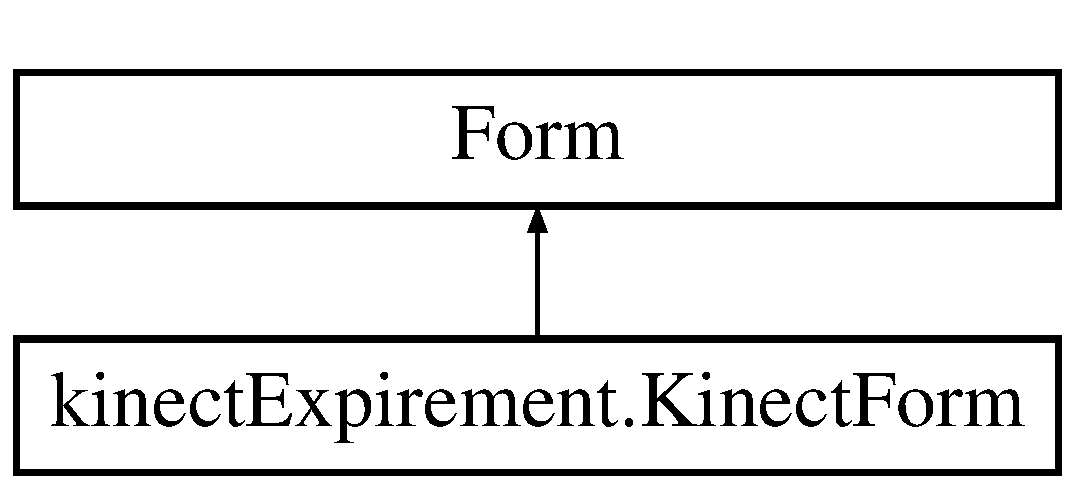
\includegraphics[height=2.000000cm]{classkinect_expirement_1_1_kinect_form}
\end{center}
\end{figure}
\subsection*{Public Member Functions}
\begin{DoxyCompactItemize}
\item 
\hyperlink{classkinect_expirement_1_1_kinect_form_abbdd0294ee8b3f1bf396ee29c5b6243a}{Kinect\+Form} ()
\begin{DoxyCompactList}\small\item\em Constructor for the \hyperlink{classkinect_expirement_1_1_kinect_form}{Kinect\+Form} class. \end{DoxyCompactList}\item 
void \hyperlink{classkinect_expirement_1_1_kinect_form_aebdf926f8e92178f1ee0c6568fb51821}{add\+Chart} (double a)
\begin{DoxyCompactList}\small\item\em Applies an offset to the value and adds it to the graph. \end{DoxyCompactList}\item 
int \hyperlink{classkinect_expirement_1_1_kinect_form_aca91adeeaacdde85a2cb3369626744cf}{placement} (double velocity)
\begin{DoxyCompactList}\small\item\em Calculates the position of the marker on the gradient. \end{DoxyCompactList}\item 
void \hyperlink{classkinect_expirement_1_1_kinect_form_a76ca898e9b3e124df1276576fbb22227}{draw} (int \hyperlink{classkinect_expirement_1_1_kinect_form_aca91adeeaacdde85a2cb3369626744cf}{placement}, Pen pen)
\begin{DoxyCompactList}\small\item\em Draws black line on the gradient. \end{DoxyCompactList}\item 
void \hyperlink{classkinect_expirement_1_1_kinect_form_aa3555a49133e17a9019c174ce96ae4c3}{erase} (int \hyperlink{classkinect_expirement_1_1_kinect_form_aca91adeeaacdde85a2cb3369626744cf}{placement})
\begin{DoxyCompactList}\small\item\em Erases the black line one the gradient. \end{DoxyCompactList}\item 
void \hyperlink{classkinect_expirement_1_1_kinect_form_a272a8bf1c0f2ec1d7e9f3260d0e351c8}{add\+Position} (double input)
\begin{DoxyCompactList}\small\item\em Adds the postion to an array and calculates the velocity. \end{DoxyCompactList}\item 
void \hyperlink{classkinect_expirement_1_1_kinect_form_a791ef370e5ae37fb90c71341cd4928ba}{set\+Button\+Enabled2} (bool value)
\begin{DoxyCompactList}\small\item\em Sets the status of the {\ttfamily btn\+Stop} button. \end{DoxyCompactList}\item 
void \hyperlink{classkinect_expirement_1_1_kinect_form_abfd5c8462b00f745fa77c19fa61d2eed}{set\+Label1} (String input)
\begin{DoxyCompactList}\small\item\em Sets the text of the {\ttfamily set\+Label1} label. \end{DoxyCompactList}\item 
void \hyperlink{classkinect_expirement_1_1_kinect_form_ac513e5db69e81ee263a5e6ad4d7029d0}{start\+Timer} ()
\begin{DoxyCompactList}\small\item\em Starts the timer for the arduino. \end{DoxyCompactList}\item 
void \hyperlink{classkinect_expirement_1_1_kinect_form_a13a559fc738ff51f58d79991b7de6146}{set\+Label\+File} (string input)
\begin{DoxyCompactList}\small\item\em Sets the text of the {\ttfamily lbl\+File\+Name} label. \end{DoxyCompactList}\item 
void \hyperlink{classkinect_expirement_1_1_kinect_form_a58486dea191eaf6b1110e655699a5ccc}{set\+Arduino\+Label} (string input)\hypertarget{classkinect_expirement_1_1_kinect_form_a58486dea191eaf6b1110e655699a5ccc}{}\label{classkinect_expirement_1_1_kinect_form_a58486dea191eaf6b1110e655699a5ccc}

\begin{DoxyCompactList}\small\item\em Sets the text of the {\ttfamily lbl\+Arduino\+Status} label.  \end{DoxyCompactList}\end{DoxyCompactItemize}
\subsection*{Public Attributes}
\begin{DoxyCompactItemize}
\item 
string \hyperlink{classkinect_expirement_1_1_kinect_form_af26c689e66a18aa21dfb11a8ec01a6dd}{time\+Start}
\begin{DoxyCompactList}\small\item\em The time stamp that the sensors start recording. \end{DoxyCompactList}\item 
string \hyperlink{classkinect_expirement_1_1_kinect_form_ae6cd686e49bc40b85ce2fdb1a053be6a}{time\+End}
\begin{DoxyCompactList}\small\item\em The time stamp that the sensors stop recording. \end{DoxyCompactList}\item 
double {\bfseries start\+Stamp}\hypertarget{classkinect_expirement_1_1_kinect_form_a97ad5d8c12f02f602249feaedc45e551}{}\label{classkinect_expirement_1_1_kinect_form_a97ad5d8c12f02f602249feaedc45e551}

\item 
bool \hyperlink{classkinect_expirement_1_1_kinect_form_a2faba08ba3886e70886d6289dcc09896}{write} = false
\begin{DoxyCompactList}\small\item\em Determines if the values read in should be written to a file. \end{DoxyCompactList}\item 
\hyperlink{classkinect_expirement_1_1_butterworth}{Butterworth} \hyperlink{classkinect_expirement_1_1_kinect_form_abec90e6db4a70d6cccc38f90f800e3ab}{angle\+\_\+butterworth} = new \hyperlink{classkinect_expirement_1_1_butterworth}{Butterworth}(\hyperlink{classkinect_expirement_1_1_butterworth_ac991123445c654cb0da7d7841e313b2c}{Butterworth.\+A\+N\+G\+LE})
\begin{DoxyCompactList}\small\item\em \hyperlink{classkinect_expirement_1_1_butterworth}{Butterworth} filter for filtering angle values. \end{DoxyCompactList}\item 
\hyperlink{classkinect_expirement_1_1_butterworth}{Butterworth} \hyperlink{classkinect_expirement_1_1_kinect_form_a7f1502bd90febb3137d8e4fdf71d52ec}{velocity\+\_\+butterworth} = new \hyperlink{classkinect_expirement_1_1_butterworth}{Butterworth}(\hyperlink{classkinect_expirement_1_1_butterworth_afc717929ffc8d554b7e0263e2b06806a}{Butterworth.\+V\+E\+L\+O\+C\+I\+TY})
\begin{DoxyCompactList}\small\item\em \hyperlink{classkinect_expirement_1_1_butterworth}{Butterworth} filter for filtering velocity values. \end{DoxyCompactList}\item 
float \hyperlink{classkinect_expirement_1_1_kinect_form_a97a0dd9256e1093328fafccaca672398}{kinect\+\_\+offset} = 0
\begin{DoxyCompactList}\small\item\em Floating point value for the offset to take of of value from the Kinect. \end{DoxyCompactList}\item 
int \hyperlink{classkinect_expirement_1_1_kinect_form_a6334825924ef2914544c0c96c0ad0572}{velocity\+\_\+goal}
\begin{DoxyCompactList}\small\item\em The desired velocity of the session. \end{DoxyCompactList}\item 
int \hyperlink{classkinect_expirement_1_1_kinect_form_aedd93118198e798ee966ff768038bac1}{velocity\+\_\+counter}
\begin{DoxyCompactList}\small\item\em Counter of how many velocity values have been calculated \end{DoxyCompactList}\item 
\hyperlink{classkinect_expirement_1_1_encoder_sensor_class}{Encoder\+Sensor\+Class} {\bfseries encoder}\hypertarget{classkinect_expirement_1_1_kinect_form_a84783ffbc816e15191e90aaab8f965c6}{}\label{classkinect_expirement_1_1_kinect_form_a84783ffbc816e15191e90aaab8f965c6}

\item 
\hyperlink{classkinect_expirement_1_1_kinect_sensor_class}{Kinect\+Sensor\+Class} {\bfseries kinect}\hypertarget{classkinect_expirement_1_1_kinect_form_a8a272c61595b87536d299d9f52ff77aa}{}\label{classkinect_expirement_1_1_kinect_form_a8a272c61595b87536d299d9f52ff77aa}

\item 
\hyperlink{classkinect_expirement_1_1_upsampler}{Upsampler} {\bfseries interp}\hypertarget{classkinect_expirement_1_1_kinect_form_af9a3d5384eda08f544c06550fa4d2774}{}\label{classkinect_expirement_1_1_kinect_form_af9a3d5384eda08f544c06550fa4d2774}

\item 
System.\+Windows.\+Forms.\+Label {\bfseries lbl\+Arduino\+Status}\hypertarget{classkinect_expirement_1_1_kinect_form_a36cbbdb03752a5ac8dc8fb6dd76973d1}{}\label{classkinect_expirement_1_1_kinect_form_a36cbbdb03752a5ac8dc8fb6dd76973d1}

\end{DoxyCompactItemize}
\subsection*{Protected Member Functions}
\begin{DoxyCompactItemize}
\item 
override void \hyperlink{classkinect_expirement_1_1_kinect_form_a906a228a66990023618b6cf919fcee44}{Dispose} (bool disposing)
\begin{DoxyCompactList}\small\item\em Clean up any resources being used. \end{DoxyCompactList}\end{DoxyCompactItemize}


\subsection{Detailed Description}
Inheriated from Form class, G\+UI for incoder and Kinect handling. 



\subsection{Constructor \& Destructor Documentation}
\index{kinect\+Expirement\+::\+Kinect\+Form@{kinect\+Expirement\+::\+Kinect\+Form}!Kinect\+Form@{Kinect\+Form}}
\index{Kinect\+Form@{Kinect\+Form}!kinect\+Expirement\+::\+Kinect\+Form@{kinect\+Expirement\+::\+Kinect\+Form}}
\subsubsection[{\texorpdfstring{Kinect\+Form()}{KinectForm()}}]{\setlength{\rightskip}{0pt plus 5cm}kinect\+Expirement.\+Kinect\+Form.\+Kinect\+Form (
\begin{DoxyParamCaption}
{}
\end{DoxyParamCaption}
)}\hypertarget{classkinect_expirement_1_1_kinect_form_abbdd0294ee8b3f1bf396ee29c5b6243a}{}\label{classkinect_expirement_1_1_kinect_form_abbdd0294ee8b3f1bf396ee29c5b6243a}


Constructor for the \hyperlink{classkinect_expirement_1_1_kinect_form}{Kinect\+Form} class. 



\subsection{Member Function Documentation}
\index{kinect\+Expirement\+::\+Kinect\+Form@{kinect\+Expirement\+::\+Kinect\+Form}!add\+Chart@{add\+Chart}}
\index{add\+Chart@{add\+Chart}!kinect\+Expirement\+::\+Kinect\+Form@{kinect\+Expirement\+::\+Kinect\+Form}}
\subsubsection[{\texorpdfstring{add\+Chart(double a)}{addChart(double a)}}]{\setlength{\rightskip}{0pt plus 5cm}void kinect\+Expirement.\+Kinect\+Form.\+add\+Chart (
\begin{DoxyParamCaption}
\item[{double}]{a}
\end{DoxyParamCaption}
)}\hypertarget{classkinect_expirement_1_1_kinect_form_aebdf926f8e92178f1ee0c6568fb51821}{}\label{classkinect_expirement_1_1_kinect_form_aebdf926f8e92178f1ee0c6568fb51821}


Applies an offset to the value and adds it to the graph. 


\begin{DoxyParams}{Parameters}
{\em a} & The orignial input value to add to the chart. \\
\hline
\end{DoxyParams}
\index{kinect\+Expirement\+::\+Kinect\+Form@{kinect\+Expirement\+::\+Kinect\+Form}!add\+Position@{add\+Position}}
\index{add\+Position@{add\+Position}!kinect\+Expirement\+::\+Kinect\+Form@{kinect\+Expirement\+::\+Kinect\+Form}}
\subsubsection[{\texorpdfstring{add\+Position(double input)}{addPosition(double input)}}]{\setlength{\rightskip}{0pt plus 5cm}void kinect\+Expirement.\+Kinect\+Form.\+add\+Position (
\begin{DoxyParamCaption}
\item[{double}]{input}
\end{DoxyParamCaption}
)}\hypertarget{classkinect_expirement_1_1_kinect_form_a272a8bf1c0f2ec1d7e9f3260d0e351c8}{}\label{classkinect_expirement_1_1_kinect_form_a272a8bf1c0f2ec1d7e9f3260d0e351c8}


Adds the postion to an array and calculates the velocity. 


\begin{DoxyParams}{Parameters}
{\em input} & Value of elbow position. \\
\hline
\end{DoxyParams}
\index{kinect\+Expirement\+::\+Kinect\+Form@{kinect\+Expirement\+::\+Kinect\+Form}!Dispose@{Dispose}}
\index{Dispose@{Dispose}!kinect\+Expirement\+::\+Kinect\+Form@{kinect\+Expirement\+::\+Kinect\+Form}}
\subsubsection[{\texorpdfstring{Dispose(bool disposing)}{Dispose(bool disposing)}}]{\setlength{\rightskip}{0pt plus 5cm}override void kinect\+Expirement.\+Kinect\+Form.\+Dispose (
\begin{DoxyParamCaption}
\item[{bool}]{disposing}
\end{DoxyParamCaption}
)\hspace{0.3cm}{\ttfamily [protected]}}\hypertarget{classkinect_expirement_1_1_kinect_form_a906a228a66990023618b6cf919fcee44}{}\label{classkinect_expirement_1_1_kinect_form_a906a228a66990023618b6cf919fcee44}


Clean up any resources being used. 


\begin{DoxyParams}{Parameters}
{\em disposing} & true if managed resources should be disposed; otherwise, false.\\
\hline
\end{DoxyParams}
\index{kinect\+Expirement\+::\+Kinect\+Form@{kinect\+Expirement\+::\+Kinect\+Form}!draw@{draw}}
\index{draw@{draw}!kinect\+Expirement\+::\+Kinect\+Form@{kinect\+Expirement\+::\+Kinect\+Form}}
\subsubsection[{\texorpdfstring{draw(int placement, Pen pen)}{draw(int placement, Pen pen)}}]{\setlength{\rightskip}{0pt plus 5cm}void kinect\+Expirement.\+Kinect\+Form.\+draw (
\begin{DoxyParamCaption}
\item[{int}]{placement, }
\item[{Pen}]{pen}
\end{DoxyParamCaption}
)}\hypertarget{classkinect_expirement_1_1_kinect_form_a76ca898e9b3e124df1276576fbb22227}{}\label{classkinect_expirement_1_1_kinect_form_a76ca898e9b3e124df1276576fbb22227}


Draws black line on the gradient. 


\begin{DoxyParams}{Parameters}
{\em placement} & The pixel postion of the line. \\
\hline
{\em pen} & The pen object that will be used to draw the line.  \\
\hline
\end{DoxyParams}
\index{kinect\+Expirement\+::\+Kinect\+Form@{kinect\+Expirement\+::\+Kinect\+Form}!erase@{erase}}
\index{erase@{erase}!kinect\+Expirement\+::\+Kinect\+Form@{kinect\+Expirement\+::\+Kinect\+Form}}
\subsubsection[{\texorpdfstring{erase(int placement)}{erase(int placement)}}]{\setlength{\rightskip}{0pt plus 5cm}void kinect\+Expirement.\+Kinect\+Form.\+erase (
\begin{DoxyParamCaption}
\item[{int}]{placement}
\end{DoxyParamCaption}
)}\hypertarget{classkinect_expirement_1_1_kinect_form_aa3555a49133e17a9019c174ce96ae4c3}{}\label{classkinect_expirement_1_1_kinect_form_aa3555a49133e17a9019c174ce96ae4c3}


Erases the black line one the gradient. 


\begin{DoxyParams}{Parameters}
{\em placement} & The pixel position of the black line. \\
\hline
\end{DoxyParams}
\index{kinect\+Expirement\+::\+Kinect\+Form@{kinect\+Expirement\+::\+Kinect\+Form}!placement@{placement}}
\index{placement@{placement}!kinect\+Expirement\+::\+Kinect\+Form@{kinect\+Expirement\+::\+Kinect\+Form}}
\subsubsection[{\texorpdfstring{placement(double velocity)}{placement(double velocity)}}]{\setlength{\rightskip}{0pt plus 5cm}int kinect\+Expirement.\+Kinect\+Form.\+placement (
\begin{DoxyParamCaption}
\item[{double}]{velocity}
\end{DoxyParamCaption}
)}\hypertarget{classkinect_expirement_1_1_kinect_form_aca91adeeaacdde85a2cb3369626744cf}{}\label{classkinect_expirement_1_1_kinect_form_aca91adeeaacdde85a2cb3369626744cf}


Calculates the position of the marker on the gradient. 


\begin{DoxyParams}{Parameters}
{\em velocity} & The velocity of the elbow movement. \\
\hline
\end{DoxyParams}
\begin{DoxyReturn}{Returns}
The pixel position of the line. 
\end{DoxyReturn}
\index{kinect\+Expirement\+::\+Kinect\+Form@{kinect\+Expirement\+::\+Kinect\+Form}!set\+Button\+Enabled2@{set\+Button\+Enabled2}}
\index{set\+Button\+Enabled2@{set\+Button\+Enabled2}!kinect\+Expirement\+::\+Kinect\+Form@{kinect\+Expirement\+::\+Kinect\+Form}}
\subsubsection[{\texorpdfstring{set\+Button\+Enabled2(bool value)}{setButtonEnabled2(bool value)}}]{\setlength{\rightskip}{0pt plus 5cm}void kinect\+Expirement.\+Kinect\+Form.\+set\+Button\+Enabled2 (
\begin{DoxyParamCaption}
\item[{bool}]{value}
\end{DoxyParamCaption}
)}\hypertarget{classkinect_expirement_1_1_kinect_form_a791ef370e5ae37fb90c71341cd4928ba}{}\label{classkinect_expirement_1_1_kinect_form_a791ef370e5ae37fb90c71341cd4928ba}


Sets the status of the {\ttfamily btn\+Stop} button. 

\index{kinect\+Expirement\+::\+Kinect\+Form@{kinect\+Expirement\+::\+Kinect\+Form}!set\+Label1@{set\+Label1}}
\index{set\+Label1@{set\+Label1}!kinect\+Expirement\+::\+Kinect\+Form@{kinect\+Expirement\+::\+Kinect\+Form}}
\subsubsection[{\texorpdfstring{set\+Label1(\+String input)}{setLabel1(String input)}}]{\setlength{\rightskip}{0pt plus 5cm}void kinect\+Expirement.\+Kinect\+Form.\+set\+Label1 (
\begin{DoxyParamCaption}
\item[{String}]{input}
\end{DoxyParamCaption}
)}\hypertarget{classkinect_expirement_1_1_kinect_form_abfd5c8462b00f745fa77c19fa61d2eed}{}\label{classkinect_expirement_1_1_kinect_form_abfd5c8462b00f745fa77c19fa61d2eed}


Sets the text of the {\ttfamily set\+Label1} label. 

\index{kinect\+Expirement\+::\+Kinect\+Form@{kinect\+Expirement\+::\+Kinect\+Form}!set\+Label\+File@{set\+Label\+File}}
\index{set\+Label\+File@{set\+Label\+File}!kinect\+Expirement\+::\+Kinect\+Form@{kinect\+Expirement\+::\+Kinect\+Form}}
\subsubsection[{\texorpdfstring{set\+Label\+File(string input)}{setLabelFile(string input)}}]{\setlength{\rightskip}{0pt plus 5cm}void kinect\+Expirement.\+Kinect\+Form.\+set\+Label\+File (
\begin{DoxyParamCaption}
\item[{string}]{input}
\end{DoxyParamCaption}
)}\hypertarget{classkinect_expirement_1_1_kinect_form_a13a559fc738ff51f58d79991b7de6146}{}\label{classkinect_expirement_1_1_kinect_form_a13a559fc738ff51f58d79991b7de6146}


Sets the text of the {\ttfamily lbl\+File\+Name} label. 

\index{kinect\+Expirement\+::\+Kinect\+Form@{kinect\+Expirement\+::\+Kinect\+Form}!start\+Timer@{start\+Timer}}
\index{start\+Timer@{start\+Timer}!kinect\+Expirement\+::\+Kinect\+Form@{kinect\+Expirement\+::\+Kinect\+Form}}
\subsubsection[{\texorpdfstring{start\+Timer()}{startTimer()}}]{\setlength{\rightskip}{0pt plus 5cm}void kinect\+Expirement.\+Kinect\+Form.\+start\+Timer (
\begin{DoxyParamCaption}
{}
\end{DoxyParamCaption}
)}\hypertarget{classkinect_expirement_1_1_kinect_form_ac513e5db69e81ee263a5e6ad4d7029d0}{}\label{classkinect_expirement_1_1_kinect_form_ac513e5db69e81ee263a5e6ad4d7029d0}


Starts the timer for the arduino. 



\subsection{Member Data Documentation}
\index{kinect\+Expirement\+::\+Kinect\+Form@{kinect\+Expirement\+::\+Kinect\+Form}!angle\+\_\+butterworth@{angle\+\_\+butterworth}}
\index{angle\+\_\+butterworth@{angle\+\_\+butterworth}!kinect\+Expirement\+::\+Kinect\+Form@{kinect\+Expirement\+::\+Kinect\+Form}}
\subsubsection[{\texorpdfstring{angle\+\_\+butterworth}{angle_butterworth}}]{\setlength{\rightskip}{0pt plus 5cm}{\bf Butterworth} kinect\+Expirement.\+Kinect\+Form.\+angle\+\_\+butterworth = new {\bf Butterworth}({\bf Butterworth.\+A\+N\+G\+LE})}\hypertarget{classkinect_expirement_1_1_kinect_form_abec90e6db4a70d6cccc38f90f800e3ab}{}\label{classkinect_expirement_1_1_kinect_form_abec90e6db4a70d6cccc38f90f800e3ab}


\hyperlink{classkinect_expirement_1_1_butterworth}{Butterworth} filter for filtering angle values. 

\index{kinect\+Expirement\+::\+Kinect\+Form@{kinect\+Expirement\+::\+Kinect\+Form}!kinect\+\_\+offset@{kinect\+\_\+offset}}
\index{kinect\+\_\+offset@{kinect\+\_\+offset}!kinect\+Expirement\+::\+Kinect\+Form@{kinect\+Expirement\+::\+Kinect\+Form}}
\subsubsection[{\texorpdfstring{kinect\+\_\+offset}{kinect_offset}}]{\setlength{\rightskip}{0pt plus 5cm}float kinect\+Expirement.\+Kinect\+Form.\+kinect\+\_\+offset = 0}\hypertarget{classkinect_expirement_1_1_kinect_form_a97a0dd9256e1093328fafccaca672398}{}\label{classkinect_expirement_1_1_kinect_form_a97a0dd9256e1093328fafccaca672398}


Floating point value for the offset to take of of value from the Kinect. 

\index{kinect\+Expirement\+::\+Kinect\+Form@{kinect\+Expirement\+::\+Kinect\+Form}!time\+End@{time\+End}}
\index{time\+End@{time\+End}!kinect\+Expirement\+::\+Kinect\+Form@{kinect\+Expirement\+::\+Kinect\+Form}}
\subsubsection[{\texorpdfstring{time\+End}{timeEnd}}]{\setlength{\rightskip}{0pt plus 5cm}string kinect\+Expirement.\+Kinect\+Form.\+time\+End}\hypertarget{classkinect_expirement_1_1_kinect_form_ae6cd686e49bc40b85ce2fdb1a053be6a}{}\label{classkinect_expirement_1_1_kinect_form_ae6cd686e49bc40b85ce2fdb1a053be6a}


The time stamp that the sensors stop recording. 

\index{kinect\+Expirement\+::\+Kinect\+Form@{kinect\+Expirement\+::\+Kinect\+Form}!time\+Start@{time\+Start}}
\index{time\+Start@{time\+Start}!kinect\+Expirement\+::\+Kinect\+Form@{kinect\+Expirement\+::\+Kinect\+Form}}
\subsubsection[{\texorpdfstring{time\+Start}{timeStart}}]{\setlength{\rightskip}{0pt plus 5cm}string kinect\+Expirement.\+Kinect\+Form.\+time\+Start}\hypertarget{classkinect_expirement_1_1_kinect_form_af26c689e66a18aa21dfb11a8ec01a6dd}{}\label{classkinect_expirement_1_1_kinect_form_af26c689e66a18aa21dfb11a8ec01a6dd}


The time stamp that the sensors start recording. 

\index{kinect\+Expirement\+::\+Kinect\+Form@{kinect\+Expirement\+::\+Kinect\+Form}!velocity\+\_\+butterworth@{velocity\+\_\+butterworth}}
\index{velocity\+\_\+butterworth@{velocity\+\_\+butterworth}!kinect\+Expirement\+::\+Kinect\+Form@{kinect\+Expirement\+::\+Kinect\+Form}}
\subsubsection[{\texorpdfstring{velocity\+\_\+butterworth}{velocity_butterworth}}]{\setlength{\rightskip}{0pt plus 5cm}{\bf Butterworth} kinect\+Expirement.\+Kinect\+Form.\+velocity\+\_\+butterworth = new {\bf Butterworth}({\bf Butterworth.\+V\+E\+L\+O\+C\+I\+TY})}\hypertarget{classkinect_expirement_1_1_kinect_form_a7f1502bd90febb3137d8e4fdf71d52ec}{}\label{classkinect_expirement_1_1_kinect_form_a7f1502bd90febb3137d8e4fdf71d52ec}


\hyperlink{classkinect_expirement_1_1_butterworth}{Butterworth} filter for filtering velocity values. 

\index{kinect\+Expirement\+::\+Kinect\+Form@{kinect\+Expirement\+::\+Kinect\+Form}!velocity\+\_\+counter@{velocity\+\_\+counter}}
\index{velocity\+\_\+counter@{velocity\+\_\+counter}!kinect\+Expirement\+::\+Kinect\+Form@{kinect\+Expirement\+::\+Kinect\+Form}}
\subsubsection[{\texorpdfstring{velocity\+\_\+counter}{velocity_counter}}]{\setlength{\rightskip}{0pt plus 5cm}int kinect\+Expirement.\+Kinect\+Form.\+velocity\+\_\+counter}\hypertarget{classkinect_expirement_1_1_kinect_form_aedd93118198e798ee966ff768038bac1}{}\label{classkinect_expirement_1_1_kinect_form_aedd93118198e798ee966ff768038bac1}


Counter of how many velocity values have been calculated 

\index{kinect\+Expirement\+::\+Kinect\+Form@{kinect\+Expirement\+::\+Kinect\+Form}!velocity\+\_\+goal@{velocity\+\_\+goal}}
\index{velocity\+\_\+goal@{velocity\+\_\+goal}!kinect\+Expirement\+::\+Kinect\+Form@{kinect\+Expirement\+::\+Kinect\+Form}}
\subsubsection[{\texorpdfstring{velocity\+\_\+goal}{velocity_goal}}]{\setlength{\rightskip}{0pt plus 5cm}int kinect\+Expirement.\+Kinect\+Form.\+velocity\+\_\+goal}\hypertarget{classkinect_expirement_1_1_kinect_form_a6334825924ef2914544c0c96c0ad0572}{}\label{classkinect_expirement_1_1_kinect_form_a6334825924ef2914544c0c96c0ad0572}


The desired velocity of the session. 

\index{kinect\+Expirement\+::\+Kinect\+Form@{kinect\+Expirement\+::\+Kinect\+Form}!write@{write}}
\index{write@{write}!kinect\+Expirement\+::\+Kinect\+Form@{kinect\+Expirement\+::\+Kinect\+Form}}
\subsubsection[{\texorpdfstring{write}{write}}]{\setlength{\rightskip}{0pt plus 5cm}bool kinect\+Expirement.\+Kinect\+Form.\+write = false}\hypertarget{classkinect_expirement_1_1_kinect_form_a2faba08ba3886e70886d6289dcc09896}{}\label{classkinect_expirement_1_1_kinect_form_a2faba08ba3886e70886d6289dcc09896}


Determines if the values read in should be written to a file. 



The documentation for this class was generated from the following files\+:\begin{DoxyCompactItemize}
\item 
Form1.\+cs\item 
Form1.\+Designer.\+cs\end{DoxyCompactItemize}

\hypertarget{classkinect_expirement_1_1_kinect_sensor_class}{}\section{kinect\+Expirement.\+Kinect\+Sensor\+Class Class Reference}
\label{classkinect_expirement_1_1_kinect_sensor_class}\index{kinect\+Expirement.\+Kinect\+Sensor\+Class@{kinect\+Expirement.\+Kinect\+Sensor\+Class}}


Holds all the functions for reading in and storeing values from the Kinect, also constrols the state of the sensor.  


\subsection*{Static Public Member Functions}
\begin{DoxyCompactItemize}
\item 
static void \hyperlink{classkinect_expirement_1_1_kinect_sensor_class_aa8b994e7fba2d8a238f95bb6830ca4f3}{Run\+Sensor} ()
\begin{DoxyCompactList}\small\item\em Opens and runs the methods for using the Kinect Sensor. \end{DoxyCompactList}\end{DoxyCompactItemize}
\subsection*{Static Public Attributes}
\begin{DoxyCompactItemize}
\item 
static Kinect\+Sensor {\bfseries sensor}\hypertarget{classkinect_expirement_1_1_kinect_sensor_class_adc9d831584e42495c1ade995e2b7296b}{}\label{classkinect_expirement_1_1_kinect_sensor_class_adc9d831584e42495c1ade995e2b7296b}

\item 
static I\+List$<$ Body $>$ {\bfseries bodies}\hypertarget{classkinect_expirement_1_1_kinect_sensor_class_afa0208c2f32b2863875380181f23a968}{}\label{classkinect_expirement_1_1_kinect_sensor_class_afa0208c2f32b2863875380181f23a968}

\item 
static bool {\bfseries first} = true\hypertarget{classkinect_expirement_1_1_kinect_sensor_class_a0849964fe5f5f578aa0acd1309f9c485}{}\label{classkinect_expirement_1_1_kinect_sensor_class_a0849964fe5f5f578aa0acd1309f9c485}

\item 
static List$<$ double $>$ {\bfseries lists} = new List$<$double$>$()\hypertarget{classkinect_expirement_1_1_kinect_sensor_class_a7ae7082005aeaaf8ac981d39fecfa466}{}\label{classkinect_expirement_1_1_kinect_sensor_class_a7ae7082005aeaaf8ac981d39fecfa466}

\item 
static List$<$ double $>$ {\bfseries velocity\+Angle} = new List$<$double$>$()\hypertarget{classkinect_expirement_1_1_kinect_sensor_class_a42a0ce3cb624cf8224a8c86353e2b453}{}\label{classkinect_expirement_1_1_kinect_sensor_class_a42a0ce3cb624cf8224a8c86353e2b453}

\item 
static int {\bfseries add\+Counter} = 0\hypertarget{classkinect_expirement_1_1_kinect_sensor_class_a83d086426821c4d842d3f82465b57ae0}{}\label{classkinect_expirement_1_1_kinect_sensor_class_a83d086426821c4d842d3f82465b57ae0}

\item 
static \hyperlink{classkinect_expirement_1_1_kinect_form}{Kinect\+Form} {\bfseries form}\hypertarget{classkinect_expirement_1_1_kinect_sensor_class_a0fc223d227f5f3f11b851738fae84be2}{}\label{classkinect_expirement_1_1_kinect_sensor_class_a0fc223d227f5f3f11b851738fae84be2}

\item 
static String {\bfseries name}\hypertarget{classkinect_expirement_1_1_kinect_sensor_class_a920f2c46b543d2b82c9698baf8b3c91f}{}\label{classkinect_expirement_1_1_kinect_sensor_class_a920f2c46b543d2b82c9698baf8b3c91f}

\item 
static \hyperlink{classkinect_expirement_1_1_file_processing}{File\+Processing} {\bfseries input}\hypertarget{classkinect_expirement_1_1_kinect_sensor_class_a05569b27d1abcbf09a4b84cd16ee5b3b}{}\label{classkinect_expirement_1_1_kinect_sensor_class_a05569b27d1abcbf09a4b84cd16ee5b3b}

\end{DoxyCompactItemize}


\subsection{Detailed Description}
Holds all the functions for reading in and storeing values from the Kinect, also constrols the state of the sensor. 



\subsection{Member Function Documentation}
\index{kinect\+Expirement\+::\+Kinect\+Sensor\+Class@{kinect\+Expirement\+::\+Kinect\+Sensor\+Class}!Run\+Sensor@{Run\+Sensor}}
\index{Run\+Sensor@{Run\+Sensor}!kinect\+Expirement\+::\+Kinect\+Sensor\+Class@{kinect\+Expirement\+::\+Kinect\+Sensor\+Class}}
\subsubsection[{\texorpdfstring{Run\+Sensor()}{RunSensor()}}]{\setlength{\rightskip}{0pt plus 5cm}static void kinect\+Expirement.\+Kinect\+Sensor\+Class.\+Run\+Sensor (
\begin{DoxyParamCaption}
{}
\end{DoxyParamCaption}
)\hspace{0.3cm}{\ttfamily [static]}}\hypertarget{classkinect_expirement_1_1_kinect_sensor_class_aa8b994e7fba2d8a238f95bb6830ca4f3}{}\label{classkinect_expirement_1_1_kinect_sensor_class_aa8b994e7fba2d8a238f95bb6830ca4f3}


Opens and runs the methods for using the Kinect Sensor. 



The documentation for this class was generated from the following file\+:\begin{DoxyCompactItemize}
\item 
C\+:/\+Users/inzuk/\+Documents/kinectc/kinect\+Expirement/Program.\+cs\end{DoxyCompactItemize}

\hypertarget{classkinect_expirement_1_1_point_holder}{}\section{kinect\+Expirement.\+Point\+Holder Class Reference}
\label{classkinect_expirement_1_1_point_holder}\index{kinect\+Expirement.\+Point\+Holder@{kinect\+Expirement.\+Point\+Holder}}


Holds the x,y and z positions of a point.  


\subsection*{Public Member Functions}
\begin{DoxyCompactItemize}
\item 
void \hyperlink{classkinect_expirement_1_1_point_holder_a8db1e89266f09909f756e9264323a7ca}{Set\+Value} (float valueX, float valueY, float valueZ)
\begin{DoxyCompactList}\small\item\em Sets the x, y, and z values of the point. \end{DoxyCompactList}\end{DoxyCompactItemize}
\subsection*{Public Attributes}
\begin{DoxyCompactItemize}
\item 
float \hyperlink{classkinect_expirement_1_1_point_holder_a170e58cf7ad5a21dd5c7a50eafbfb0e8}{x} = 0
\begin{DoxyCompactList}\small\item\em The x positon of the point. \end{DoxyCompactList}\item 
float \hyperlink{classkinect_expirement_1_1_point_holder_a8e1920f1bd56b015aeae9f19a6f0c5e6}{y} = 0
\begin{DoxyCompactList}\small\item\em The y position of the point. \end{DoxyCompactList}\item 
float \hyperlink{classkinect_expirement_1_1_point_holder_aa89b5a93efd8f6f6eb033ea7160c5d97}{z} = 0
\begin{DoxyCompactList}\small\item\em The z position of the point. \end{DoxyCompactList}\end{DoxyCompactItemize}


\subsection{Detailed Description}
Holds the x,y and z positions of a point. 



\subsection{Member Function Documentation}
\index{kinect\+Expirement\+::\+Point\+Holder@{kinect\+Expirement\+::\+Point\+Holder}!Set\+Value@{Set\+Value}}
\index{Set\+Value@{Set\+Value}!kinect\+Expirement\+::\+Point\+Holder@{kinect\+Expirement\+::\+Point\+Holder}}
\subsubsection[{\texorpdfstring{Set\+Value(float value\+X, float value\+Y, float value\+Z)}{SetValue(float valueX, float valueY, float valueZ)}}]{\setlength{\rightskip}{0pt plus 5cm}void kinect\+Expirement.\+Point\+Holder.\+Set\+Value (
\begin{DoxyParamCaption}
\item[{float}]{valueX, }
\item[{float}]{valueY, }
\item[{float}]{valueZ}
\end{DoxyParamCaption}
)}\hypertarget{classkinect_expirement_1_1_point_holder_a8db1e89266f09909f756e9264323a7ca}{}\label{classkinect_expirement_1_1_point_holder_a8db1e89266f09909f756e9264323a7ca}


Sets the x, y, and z values of the point. 


\begin{DoxyParams}{Parameters}
{\em valueX} & The x position of the point. $<$/params$>$ 
\begin{DoxyParams}{Parameters}
{\em valueY} & The y position of the point. $<$/params$>$ 
\begin{DoxyParams}{Parameters}
{\em valueZ} & The z position of the point. $<$/params$>$ \\
\hline
\end{DoxyParams}
\\
\hline
\end{DoxyParams}
\\
\hline
\end{DoxyParams}


\subsection{Member Data Documentation}
\index{kinect\+Expirement\+::\+Point\+Holder@{kinect\+Expirement\+::\+Point\+Holder}!x@{x}}
\index{x@{x}!kinect\+Expirement\+::\+Point\+Holder@{kinect\+Expirement\+::\+Point\+Holder}}
\subsubsection[{\texorpdfstring{x}{x}}]{\setlength{\rightskip}{0pt plus 5cm}float kinect\+Expirement.\+Point\+Holder.\+x = 0}\hypertarget{classkinect_expirement_1_1_point_holder_a170e58cf7ad5a21dd5c7a50eafbfb0e8}{}\label{classkinect_expirement_1_1_point_holder_a170e58cf7ad5a21dd5c7a50eafbfb0e8}


The x positon of the point. 

\index{kinect\+Expirement\+::\+Point\+Holder@{kinect\+Expirement\+::\+Point\+Holder}!y@{y}}
\index{y@{y}!kinect\+Expirement\+::\+Point\+Holder@{kinect\+Expirement\+::\+Point\+Holder}}
\subsubsection[{\texorpdfstring{y}{y}}]{\setlength{\rightskip}{0pt plus 5cm}float kinect\+Expirement.\+Point\+Holder.\+y = 0}\hypertarget{classkinect_expirement_1_1_point_holder_a8e1920f1bd56b015aeae9f19a6f0c5e6}{}\label{classkinect_expirement_1_1_point_holder_a8e1920f1bd56b015aeae9f19a6f0c5e6}


The y position of the point. 

\index{kinect\+Expirement\+::\+Point\+Holder@{kinect\+Expirement\+::\+Point\+Holder}!z@{z}}
\index{z@{z}!kinect\+Expirement\+::\+Point\+Holder@{kinect\+Expirement\+::\+Point\+Holder}}
\subsubsection[{\texorpdfstring{z}{z}}]{\setlength{\rightskip}{0pt plus 5cm}float kinect\+Expirement.\+Point\+Holder.\+z = 0}\hypertarget{classkinect_expirement_1_1_point_holder_aa89b5a93efd8f6f6eb033ea7160c5d97}{}\label{classkinect_expirement_1_1_point_holder_aa89b5a93efd8f6f6eb033ea7160c5d97}


The z position of the point. 



The documentation for this class was generated from the following file\+:\begin{DoxyCompactItemize}
\item 
Program.\+cs\end{DoxyCompactItemize}

\hypertarget{classkinect_expirement_1_1_upsampler}{}\section{kinect\+Expirement.\+Upsampler Class Reference}
\label{classkinect_expirement_1_1_upsampler}\index{kinect\+Expirement.\+Upsampler@{kinect\+Expirement.\+Upsampler}}
\subsection*{Public Member Functions}
\begin{DoxyCompactItemize}
\item 
\hyperlink{classkinect_expirement_1_1_upsampler_a34afdc7c65522bb74f4db79528364516}{Upsampler} ()
\begin{DoxyCompactList}\small\item\em Default constructor for the {\ttfamily \hyperlink{classkinect_expirement_1_1_upsampler}{Upsampler}} class. \end{DoxyCompactList}\item 
List$<$ double $>$ \hyperlink{classkinect_expirement_1_1_upsampler_a554b4fc6c3ba7673c5e61685efee80e2}{Down\+Sample} (ref List$<$ double $>$ samples, int desired\+\_\+frequency, int duration)
\item 
List$<$ double $>$ {\bfseries Up\+Sample} (ref List$<$ double $>$ samples, int desired\+\_\+frequency, int duration)\hypertarget{classkinect_expirement_1_1_upsampler_aaf30cd9bbed77b0f907c59a22482da8c}{}\label{classkinect_expirement_1_1_upsampler_aaf30cd9bbed77b0f907c59a22482da8c}

\end{DoxyCompactItemize}


\subsection{Constructor \& Destructor Documentation}
\index{kinect\+Expirement\+::\+Upsampler@{kinect\+Expirement\+::\+Upsampler}!Upsampler@{Upsampler}}
\index{Upsampler@{Upsampler}!kinect\+Expirement\+::\+Upsampler@{kinect\+Expirement\+::\+Upsampler}}
\subsubsection[{\texorpdfstring{Upsampler()}{Upsampler()}}]{\setlength{\rightskip}{0pt plus 5cm}kinect\+Expirement.\+Upsampler.\+Upsampler (
\begin{DoxyParamCaption}
{}
\end{DoxyParamCaption}
)}\hypertarget{classkinect_expirement_1_1_upsampler_a34afdc7c65522bb74f4db79528364516}{}\label{classkinect_expirement_1_1_upsampler_a34afdc7c65522bb74f4db79528364516}


Default constructor for the {\ttfamily \hyperlink{classkinect_expirement_1_1_upsampler}{Upsampler}} class. 

summary$>$ Down samples the an array of values to a certain frequency. 

param name = \char`\"{}samples\char`\"{}$>$ The list of data to be modified. 

param name = \char`\"{}desired\+\_\+frequency\char`\"{}$>$ The frequency the list will be changed to. 

param name = \char`\"{}duration\char`\"{}$>$ The duratiion that the data was collected. 

returns$>$ A list of doubles, down sampled to the desired frequency. 

\subsection{Member Function Documentation}
\index{kinect\+Expirement\+::\+Upsampler@{kinect\+Expirement\+::\+Upsampler}!Down\+Sample@{Down\+Sample}}
\index{Down\+Sample@{Down\+Sample}!kinect\+Expirement\+::\+Upsampler@{kinect\+Expirement\+::\+Upsampler}}
\subsubsection[{\texorpdfstring{Down\+Sample(ref List$<$ double $>$ samples, int desired\+\_\+frequency, int duration)}{DownSample(ref List< double > samples, int desired_frequency, int duration)}}]{\setlength{\rightskip}{0pt plus 5cm}List$<$double$>$ kinect\+Expirement.\+Upsampler.\+Down\+Sample (
\begin{DoxyParamCaption}
\item[{ref List$<$ double $>$}]{samples, }
\item[{int}]{desired\+\_\+frequency, }
\item[{int}]{duration}
\end{DoxyParamCaption}
)}\hypertarget{classkinect_expirement_1_1_upsampler_a554b4fc6c3ba7673c5e61685efee80e2}{}\label{classkinect_expirement_1_1_upsampler_a554b4fc6c3ba7673c5e61685efee80e2}
summary$>$ Up samples the an array of values to a certain frequency. 

param name = \char`\"{}samples\char`\"{}$>$ The list of data to be modified. 

param name = \char`\"{}desired\+\_\+frequency\char`\"{}$>$ The frequency the list will be changed to. 

param name = \char`\"{}duration\char`\"{}$>$ The duratiion that the data was collected. 

returns$>$ A list of doubles, up sampled to the desired frequency. 

The documentation for this class was generated from the following file\+:\begin{DoxyCompactItemize}
\item 
Upsampler.\+cs\end{DoxyCompactItemize}

%--- End generated contents ---

% Index
\backmatter
\newpage
\phantomsection
\clearemptydoublepage
\addcontentsline{toc}{chapter}{Index}
\printindex

\end{document}
